\documentclass{labo}
\usepackage[utf8x]{inputenc}

\usepackage[english]{babel}
\usepackage[T1]{fontenc}

\usepackage{graphicx}
\usepackage{amssymb}
\usepackage{amsmath}
\usepackage{siunitx}
\usepackage{wasysym} %smiley
\usepackage{textcomp}
% \usepackage{minted}
\usepackage[long]{datetime}
\usepackage{gensymb} % \ohm, celsius
\usepackage{framed}
\usepackage{pdfpages}
\usepackage{paralist}

\usepackage{mathastext} % math as standfard text : units are respecting typography conventions.
\usepackage{fancyhdr} %en-tête
\usepackage{qrcode}
\usepackage{pgfplots} %for latex grid
\usepackage{fontawesome}
\usepackage{charter}
\usepackage{subfig}

\usepackage{minted}

%%%%%%%%%%%%
% Tables
%%%%%%%%%%%%
\usepackage{dcolumn}
\newcolumntype{.}{D{.}{.}{2}}
\usepackage{booktabs}
\renewcommand{\arraystretch}{1.1} % Opens up the table a tad
\usepackage{multicol}
\usepackage{multirow}

\langexam{frenchb}

\correction{false}
%\correction{true}

\author{}


%% fancy header & foot
\pagestyle{fancy}
\lhead{[4EISA] Image Processing\\ LAB 3 \ifthenelse{\boolean{corrige}}{~-- correction}{}}
\rhead{v1.0.1\\ page \thepage}
\cfoot{}
%%

\pdfinfo{
/Author ()
/Title (4EISA Image Processing, lab 3)
/ModDate (D:\pdfdate)
}

\hypersetup{
pdftitle={LAB 3 [4EISA] Image Processing},
pdfauthor={},
pdfsubject={}
}

\newcommand{\numpy}{\texttt{NumPy} }
\newcommand{\opencv}{\texttt{OpenCV} }

\setminted[python]{
frame=lines,
framesep=2mm,
% baselinestretch=1.2,
fontsize=\small,
linenos
}

\begin{document}

\tptitle{}{Image Processing -- Session 3\\}

In this session, you will get into practical applications of openCV operations applied on the camera feed.

\section*{}



\section*{Green screen chroma key}
Chroma key is a special effect and a post-production technique in which multiple images can be combined together. 
This technique is widely used to replace green or blue backgrounds in an image with another image or live video to create special effects in live action or animation movies and weather forecasting. 
The logic on which the chroma key technique is based is very simple: we use a uniform-coloured background, usually bright green or blue, and then replace that with an image or another live video.

Start by importing the needed packages and initialising the capture:
\begin{minted}{python}
import numpy as np
import cv2

cam = cv2.VideoCapture(0)
\end{minted}

You can lower the camera resolution to try to get a better frame rate:
\begin{minted}{python}
cam.set(3,640)
cam.set(4,480)
\end{minted}

Let's say your subject is taken on a relatively uniform background as illustrated on Figure~\ref{fig:pink-bg}.


You can get that feed from the camera or load it from file:
\begin{minted}{python}
while(true):
	ret, frame = cam.read() # From the camera
frame = cv2.imread("akabeko-pink-bg.png") # From a static image
\end{minted}

As we saw previously, the  HSV colour format is the most appropriate format for any type of activity that involves operation on a range of colours; we will convert the image into the HSV format and calculate the mask for the green background, as follows:
\begin{minted}{python}
hsv = cv2.cvtColor(frame, cv2.COLOR_BGR2HSV)
image_mask = cv2.inRange(hsv, np.array([5,80,150]), np.array([6,100,200]))
\end{minted}

The image mask will appear as on Figure\ref{fig:pink-bg-mask}, where pink pixels are replaced by the colour white and others are assigned the colour black.


Once we have obtained the background image mask, we can easily apply it on the background image to obscure the foreground object with black pixels as follows:
\begin{minted}{python}
bg_mask = cv2.bitwise_and(bg,bg,mask=image_mask)
\end{minted}

The result will replace all the white pixels with the background image and the foreground area will still have the black pixels, as seen here on Figure~\ref{fig:bg-mask}.


Now, we need to extract only the foreground image from our camera feed or original image. This can be accomplished by using the following code:
\begin{minted}{python}
fg_mask = cv2.bitwise_and(frame,frame,mask = cv2.bitwise_not(image_mask))
\end{minted}
This will extract all the non-green objects, while assigning the colour black to the pixels corresponding to the green background.

Finally, we will add our last two image outputs, which will provide us with the required chroma key effect, by replacing the green screen with the custom background on Figure~\ref{fig:akabeko-space-bg}.
\begin{minted}{python}
cv2.imshow('Output',cv2.add(bg_mask,fg_mask))
if cv2.waitKey(1) == 27:
	break
cv2.destroyAllWindows()
cam.release()
\end{minted}


\begin{figure}[h]
\centering
\subfloat[Original image\label{fig:pink-bg}]{%
	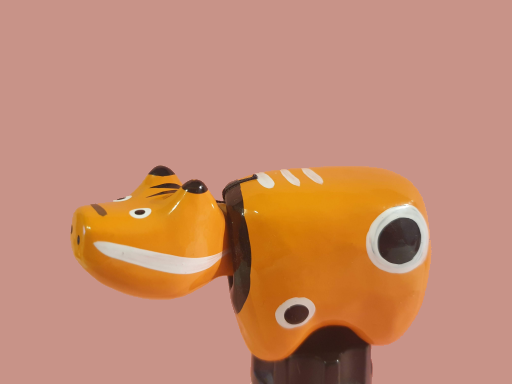
\includegraphics[width=.45\textwidth]{akabeko-pink-bg.png}%
}
\hfill
\subfloat[Background removed\label{fig:pink-bg-mask}]{%
	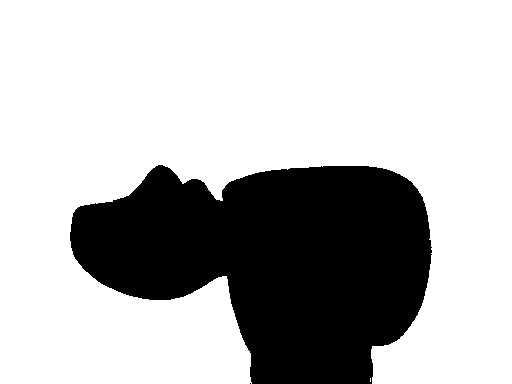
\includegraphics[width=.45\textwidth]{akabeko-pink-bg-mask}%
}\\

\subfloat[Original image masked on the new background\label{fig:bg-mask}]{%
	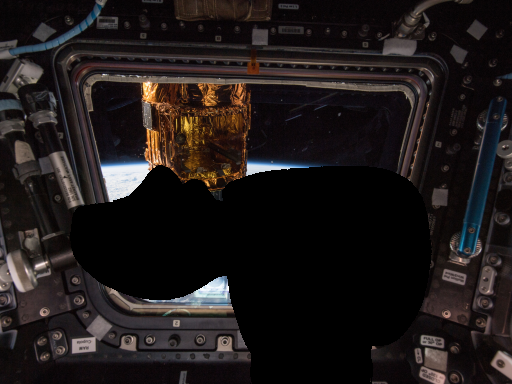
\includegraphics[width=.45\textwidth]{bg-mask.png}%
}
\hfill
\subfloat[Original image with the background replaced\label{fig:akabeko-space-bg}]{%
	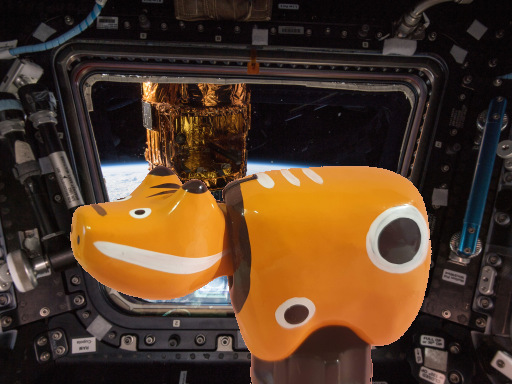
\includegraphics[width=.45\textwidth]{akabeko-space-bg.png}%
}
\caption{}
\label{fig:clust-hier-geo}
\end{figure}





\section*{Motion detection and tracking}
We will now build a sophisticated motion detection and tracking system with a very simple logic of finding the difference between subsequent frames from a video feed, like a webcam stream, and plotting contours around the area where the difference is detected.
Let's import the required libraries and initialize the webcam:
\begin{minted}{python}
import cv2
import numpy as np
cap = cv2.VideoCapture(0)
\end{minted}

We will need a kernel for the dilation operation, which we will create in advance, rather than creating it every time in the loop:
\begin{minted}{python}
k = np.ones((3,3),np.uint8)
\end{minted}

The following code will capture and store subsequent frames:
\begin{minted}{python}
t0 = cap.read()[1]
t1 = cap.read()[1]
\end{minted}

Now, we will initiate the while loop and calculate the difference between both frames, and then convert the output to greyscale for further processing:
\begin{minted}{python}
while(True):
	d = cv2.absdiff(t1,t0)
	grey = cv2.cvtColor(d, cv2.COLOR_BGR2GRAY)
\end{minted}

The output will be as Figure~\ref{fig:motion-base}, showing the difference of pixels between the frames.
\begin{figure}[ht!]
\centering
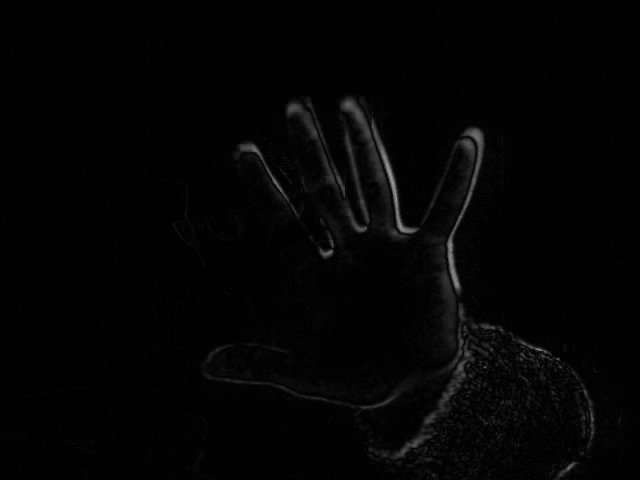
\includegraphics[width=.7\textwidth]{motion-grey.png}
\caption{}
\label{fig:motion-base}
\end{figure}

This image may contain some noise, so we will blur it first:
\begin{minted}{python}
blur = cv2.GaussianBlur(grey,(3,3),0)
\end{minted}
We use the binary threshold to convert this noise-removed output into a binary image with the following code:
\begin{minted}{python}
ret, th = cv2.threshold(blur, 15, 255, cv2.THRESH_BINARY)
\end{minted}
The final operation is to dilate the image so that it is easier for us to find the boundary clearly:
\begin{minted}{python}
dilated = cv2.dilate(th,k,iterations=2)
\end{minted}
The output of the preceding step is shown on Figure~\ref{fig:motion-filter}.

\begin{figure}[ht!]
\centering
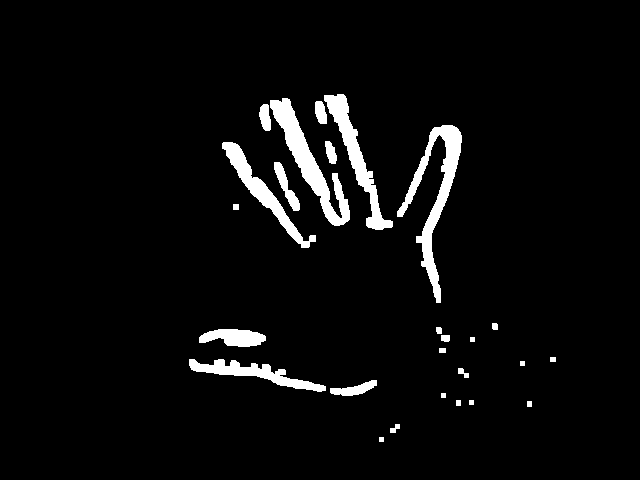
\includegraphics[width=.7\textwidth]{motion-dilated.png}
\caption{}
\label{fig:motion-filter}
\end{figure}

Then, we will find and draw the contours for the preceding image with the following code:
\begin{minted}{python}
contours, hierarchy = cv2.findContours(dilated,cv2.RETR_TREE,cv2.CHAIN_APPROX_SIMPLE)
t2 = t0
cv2.drawContours(t2, contours, -1, (0,255,0), 2 )
cv2.imshow('Output', t2)
\end{minted}

Finally, we will assign the latest frame to the older frame and capture the next frame with a webcam:
\begin{minted}{python}
t0 = t1
t1 = cap.read()[1]
\end{minted}

We will terminate the loop once we detect the \texttt{Esc} keypress, as usual:
\begin{minted}{python}
if cv2.waitKey(5) == 27 :
	break
\end{minted}
Once the loop is terminated, we will release the camera and destroy the display window:
\begin{minted}{python}
cap.release()
cv2.destroyAllWindows()
\end{minted}
This will draw the contour roughly around the area where the movement is detected, as seen on Figure~\ref{fig:motion-contour}.

\begin{figure}[ht!]
\centering
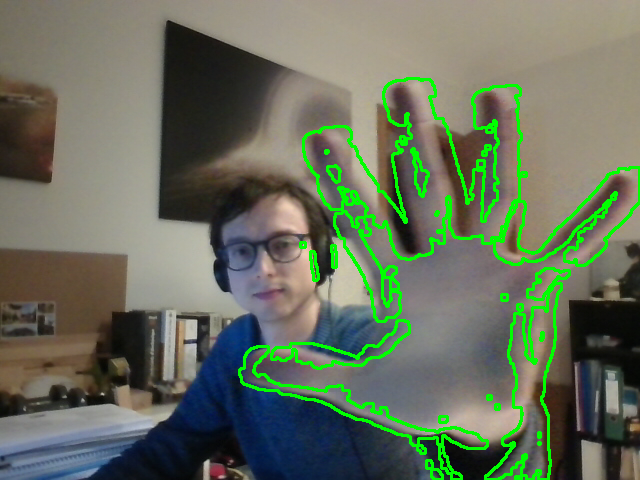
\includegraphics[width=.7\textwidth]{motion-contour.png}
\caption{A moving hand motion has been detected.}
\label{fig:motion-contour}
\end{figure}
This code works very well for slow movements. You can make the output more interesting by drawing contours with different colours. Also, you can find out the centroid of the contours and draw crosshairs or circles corresponding to the centroids.





% In this session, you will be able to obtain more details about a picture and interact with the raspberry Pi through the PiCamera.

% \section*{Restoring images using inpainting}
% Image restoration is the process of reconstructing the damaged parts of an image. In digital images, data errors can be introduced in an image during the transmission and reception. For example, when images are transmitted byte by byte (instead of packets), it is not feasible to use modern error checking and corrective networking protocols, which increases the probability of getting erroneous data. Many of these degraded images can be restored using the image \textbf{inpainting} technique. There are several algorithms available for the same, and OpenCV offers two of these with its \texttt{cv2.inpaint()} function\footnote{\texttt{cv2.INPAINT\_TELEA} is based on the paper \textit{An Image Inpainting Technique Based on the Fast Marching Method} by Alexandru Telea published in 2004 (\href{http://dx.doi.org/10.1080/10867651.2004.10487596}{10.1080/10867651.2004.10487596}), and \texttt{cv2.INPAINT\_NS} is based on \textit{Navier-Stokes, Fluid Dynamics, and Image and Video Inpainting}, by Bertalmio, Marcelo, Andrea L. Bertozzi, and Guillermo Sapiro published in 2001 (\href{http://dx.doi.org/10.1109/CVPR.2001.990497}{10.1109/CVPR.2001.990497}).}.\\

% It accepts a source image, an \textit{inpaint} mask that is a greyscale image representation of the damaged area where the non-zero (white) pixels denote the area to be inpainted, an inpaint neighbourhood side, and an algorithm that has to be applied as parameters. The function then returns the inpainted image. The following code demonstrates the implementation of both of these methods that are available in \opencv for inpainting. The results are almost the same in both the algorithms. We manually created the damage and the corresponding mask (by inverting the damage pixels) in an image manipulation software:

% \begin{minted}{python}
% import cv2 
% import matplotlib.pyplot as plt 
% image = cv2.imread('degraded.png') 
% mask = cv2.imread('msk.png',0) 
% input_img = cv2.cvtColor( image , cv2.COLOR_BGR2RGB ) 
% output_TELEA = cv2.inpaint(input_img,mask,5,cv2.INPAINT_TELEA) 
% output_NS = cv2.inpaint(input_img,mask,5,cv2.INPAINT_NS) 
% titles = ['Damaged Image', 'Mask', 'Telea Method', 'Navier Stokes Method']
% images = [input_img, mask, output_TELEA, output_NS
% for i in range(len(titles)):
% 	plt.subplot(221+i)
% 	if titles[i] == 'Mask':
% 		plt.imshow(images[i],cmap='gray')
% 	else:
% 		plt.imshow(images[i])
% 	plt.imshow(images[i])
% 	plt.title(titles[i])
% 	plt.xticks([])
% 	plt.yticks([]) 
% plt.show()
% \end{minted}





% \section*{K-means clustering and image quantisation}
% The k-means clustering algorithm is a quantisation algorithm that maps sets of values within a range into a cluster determined by a value (mean). It basically divides a given set of n values into k partitions. This is called clustering when it's applied on data with two or more dimensions. \opencv has \texttt{cv2.kmeans()} for the implementation of the k-means algorithm. It accepts the following parameters:
% \begin{itemize}
% 	\item Data: This is the data that has to be clustered. If we provide an image, the output will be a quantised (segmented) image. This has to be in the float format. 
% 	\item K: This is the number of partitions in the output set (it is the number of colours in the output if the input is an image). 
% 	\item Criteria: This is the algorithm termination criteria that includes a number of iterations and/or the desired accuracy. 
% 	\item Attempts: This is the number of times the algorithms will be executed using a different initial labelling. 
% 	\item Flags: These specify the initial centres of the clusters, which can have any of the following values: \texttt{cv2.KMEANS\_RANDOM\_CENTERS}, \texttt{cv2.KMEANS\_PP\_CENTERS} or \texttt{cv2.KMEANS\_USE\_INITIAL\_LABELS}.
% \end{itemize}

% \begin{minted}{python}
% import cv2 
% import numpy as np 
% import matplotlib.pyplot as plt 
% image=cv2.imread('italy.png') 
% input_img = cv2.cvtColor(image,cv2.COLOR_BGR2RGB) 
% Z = input_img.reshape((-1,3)) 
% Z = np.float32(Z) 
% criteria = (cv2.TERM_CRITERIA_EPS + cv2.TERM_CRITERIA_MAX_ITER,10,1.0) 
% K = 2 
% ret,label1,center1 = cv2.kmeans(Z,K,none,criteria,10,cv2.KMEANS_RANDOM_CENTERS) 
% center1 = np.uint8(center1) 
% res1 = center1[label1.flatten()] 
% output1 = res1.reshape((image.shape)) 
% K = 4 
% ret,label2,center2 = cv2.kmeans(Z,K,none,criteria,10,cv2.KMEANS_RANDOM_CENTERS) 
% center2 = np.uint8(center2) 
% res2 = center2[label2.flatten()] 
% output2 = res2.reshape((image.shape)) 
% K = 8 
% ret,label3,center3 = cv2.kmeans(Z,K,none,criteria,10,cv2.KMEANS_RANDOM_CENTERS) 
% center3 = np.uint8(center3) 
% res3 = center3[label3.flatten()] 
% output3 = res3.reshape((image.shape)) 
% titles = ['Original','K=2','K=4','K=8'] 
% output = [input_img,output1,output2,output3] 
% for i in range(4): 
% 	plt.subplot(2,2,i+1)
% 	plt.imshow(output[i])
% 	plt.title(titles[i]) 
% 	plt.xticks([])
% 	plt.yticks([]) 
% plt.show()
% \end{minted}

% We initially assigned random centres to all the clusters with the \texttt{cv2.KMEANS\_RANDOM\_CENTERS} flag. The output of the preceding program will be the original image with the quantized and segmented images, with 2, 4, and 8 colours\footnote{The execution time might be longer than usual (over a few minutes).}. 
% \begin{leftbar}
% As an exercise, try using the algorithm with different sets and combinations of inputs and compare the results.
% \end{leftbar}

% \section*{Disparity map and depth estimation}
% Disparity refers to the difference in the location of an object in the corresponding two (left and right) images as seen by the left and right eye, which is created due to a parallax. Our brain uses this disparity to estimate the depth information from the pair of two-dimensional images. We can calculate the disparity between the two images by applying this principle to every pixel in the pair of images. Once we have the disparity information, we can leverage it to estimate the depth just the way our brain uses it to estimate depth. In biology, this is called stereoscopic vision. OpenCV provides the \texttt{cv2.StereoBM.compute()} function, which takes the left image and the right image as a parameter and returns the disparity map of the image pair. The \texttt{cv2.StereoBM()} function is the constructor that initializes the stereo state. It accepts a preset, the number of disparities (which is a multiple of 16), and \texttt{SADWindowSize}, which is a linear block size for comparison. This stereo state is implicitly used to compute disparity map by \texttt{cv2.StereoBM.compute()}.

% \begin{minted}{python}
% import cv2 
% import numpy as np 
% import matplotlib.pyplot as plt 
% Right = cv2.imread('img4.png',0) 
% Left = cv2.imread('img3.png',0) 
% stereo_BM_state = cv2.StereoBM_create(numDisparities=32, blockSize=27)
% output_map = stereo_BM_state.compute(Left,Right) 
% titles = ['Left','Right','Depth Map'] 
% output = [Left,Right,output_map] 
% for i in range(3): 
% 	plt.subplot(1,3,i+1)
% 	plt.imshow(output[i],cmap='gray') 
% 	plt.title(titles[i]) 
% 	plt.xticks([])
% 	plt.yticks([]) 
% plt.show()
% \end{minted}

% A smaller \texttt{SADWindowSize} value will provide a detailed but distorted map, and a higher value will provide a smoother map, as seen in the preceding output. 
% \begin{leftbar}
% As an exercise, try out different values of \texttt{ndisparities} and \texttt{SADWindowSize}. \texttt{SADWindowSize} has to be an odd positive value. 
% \end{leftbar}

% In the preceding image, the brighter areas denote more disparity, which means that the objects in the input images corresponding to the brighter areas in the output image are closer to the cameras. In the same way, the darker colours in the disparity map mean that the corresponding objects in the images are farther from the camera.




% \section*{Image histograms}
% A histogram is a way to graphically represent the distribution of data. An image histogram is the representation of an image array. It represents the tonal distribution of the digital image. Basically, the histogram of an image is a graphical representation of the distribution of colour or luminance variance in an image. In an image histogram, the x axis represents the variation of colours, and the y axis represents the total number of pixels for a particular colour tone. If we were to plot a histogram for a greyscale image, the x axis will represent the different intensity values (0 to 255, for example), and the y axis will represent the number of pixels that have such values.\\

% In a similar way, we can plot the histogram for colour images by plotting the image histogram for each channel (red, green, and blue, for example). Let's get started by plotting a histogram of a greyscale image. We will use the hist() function that belongs to the \texttt{matplotlib} library. Run the following code:

% \begin{minted}{python}
% import cv2 
% import matplotlib.pyplot as plt 
% img = cv2.imread('parrots.bmp',0) 
% plt.hist(img.ravel(),256,[0,256]) 
% plt.show()
% \end{minted}

% In the preceding code, we passed an image, the number of vertical edges in the histogram, and a range as an argument to the \texttt{plt.hist()} function. You can pass more arguments to this function\footnote{Full doc online: \url{https://matplotlib.org/stable/api/_as_gen/matplotlib.pyplot.html}}.\\

% \opencv also has a function to plot histograms for colour images. The \texttt{cv2.calcHist()} function accepts an image, channel, mask, size, and range as arguments. The following example shows its usage by plotting a histogram for each channel (red, green, and blue):

% \begin{minted}{python}
% import cv2 
% import matplotlib.pyplot as plt 
% img = cv2.imread('parrots.bmp',1) 
% input_img = cv2.cvtColor(img,cv2.COLOR_RGB2BGR) 
% histr_RED = cv2.calcHist([input_img],[0],None,[256],[0,256]) 
% histr_GREEN = cv2.calcHist([input_img],[1],None,[256],[0,256]) 
% histr_BLUE = cv2.calcHist([input_img],[2],None,[256],[0,256]) 
% titles = ['Red', 'Green', 'Blue']
% histograms = [histr_RED, histr_GREEN, histr_BLUE]
% colours = ['r', 'g', 'b']
% plt.subplot(221)
% plt.imshow(input_img)
% plt.title('Original Image')
% plt.xticks([])
% plt.yticks([]) 
% for i in range(len(titles)):
% 	plt.subplot(222+i)
% 	plt.plot(histograms[i],color=colours[i]) 
% 	plt.title(titles[i]) 
% 	plt.xlim([0,256])
% 	plt.yticks([])
% plt.show()
% \end{minted}

% \section*{Image contours}








% \begin{minted}{python}

% \end{minted}

%\Question{}{}
\end{document}
